% Options for packages loaded elsewhere
\PassOptionsToPackage{unicode}{hyperref}
\PassOptionsToPackage{hyphens}{url}
\PassOptionsToPackage{dvipsnames,svgnames,x11names}{xcolor}
%
\documentclass[
  12pt,
  letterpaper,
  DIV=11,
  numbers=noendperiod]{scrartcl}

\usepackage{amsmath,amssymb}
\usepackage{lmodern}
\usepackage{iftex}
\ifPDFTeX
  \usepackage[T1]{fontenc}
  \usepackage[utf8]{inputenc}
  \usepackage{textcomp} % provide euro and other symbols
\else % if luatex or xetex
  \usepackage{unicode-math}
  \defaultfontfeatures{Scale=MatchLowercase}
  \defaultfontfeatures[\rmfamily]{Ligatures=TeX,Scale=1}
\fi
% Use upquote if available, for straight quotes in verbatim environments
\IfFileExists{upquote.sty}{\usepackage{upquote}}{}
\IfFileExists{microtype.sty}{% use microtype if available
  \usepackage[]{microtype}
  \UseMicrotypeSet[protrusion]{basicmath} % disable protrusion for tt fonts
}{}
\makeatletter
\@ifundefined{KOMAClassName}{% if non-KOMA class
  \IfFileExists{parskip.sty}{%
    \usepackage{parskip}
  }{% else
    \setlength{\parindent}{0pt}
    \setlength{\parskip}{6pt plus 2pt minus 1pt}}
}{% if KOMA class
  \KOMAoptions{parskip=half}}
\makeatother
\usepackage{xcolor}
\usepackage[margin=1in]{geometry}
\setlength{\emergencystretch}{3em} % prevent overfull lines
\setcounter{secnumdepth}{5}
% Make \paragraph and \subparagraph free-standing
\ifx\paragraph\undefined\else
  \let\oldparagraph\paragraph
  \renewcommand{\paragraph}[1]{\oldparagraph{#1}\mbox{}}
\fi
\ifx\subparagraph\undefined\else
  \let\oldsubparagraph\subparagraph
  \renewcommand{\subparagraph}[1]{\oldsubparagraph{#1}\mbox{}}
\fi


\providecommand{\tightlist}{%
  \setlength{\itemsep}{0pt}\setlength{\parskip}{0pt}}\usepackage{longtable,booktabs,array}
\usepackage{calc} % for calculating minipage widths
% Correct order of tables after \paragraph or \subparagraph
\usepackage{etoolbox}
\makeatletter
\patchcmd\longtable{\par}{\if@noskipsec\mbox{}\fi\par}{}{}
\makeatother
% Allow footnotes in longtable head/foot
\IfFileExists{footnotehyper.sty}{\usepackage{footnotehyper}}{\usepackage{footnote}}
\makesavenoteenv{longtable}
\usepackage{graphicx}
\makeatletter
\def\maxwidth{\ifdim\Gin@nat@width>\linewidth\linewidth\else\Gin@nat@width\fi}
\def\maxheight{\ifdim\Gin@nat@height>\textheight\textheight\else\Gin@nat@height\fi}
\makeatother
% Scale images if necessary, so that they will not overflow the page
% margins by default, and it is still possible to overwrite the defaults
% using explicit options in \includegraphics[width, height, ...]{}
\setkeys{Gin}{width=\maxwidth,height=\maxheight,keepaspectratio}
% Set default figure placement to htbp
\makeatletter
\def\fps@figure{htbp}
\makeatother

% variáveis
\newcommand{\nome}{Alberson da Silva}
\newcommand{\sobrenome}{Miranda}
\newcommand{\tipo}{Dissertação}
\newcommand{\tipoingles}{Thesis}
\newcommand{\titulo}{Reconciliação Ótima Probabilística em Séries Temporais Hierárquicas}
\newcommand{\tituloingles}{Probabilistic Optimal Conciliation of Hierarquic Time Series}
\newcommand{\universidade}{Universidade Federal do Espírito Santo}
\newcommand{\campus}{Centro de Ciências Jurídicas e Econômicas}
\newcommand{\curso}{Programa de Pós-Graduação em Economia}
\newcommand{\cursoingles}{MSc. in Economics}
\newcommand{\orientador}{Prof. Dr. Guilherme A. A. Pereira}
\newcommand{\cidade}{Vitória}
\newcommand{\dia}{xx}
\newcommand{\mes}{setembro}
\newcommand{\ano}{2022}
\newcommand{\grau}{Mestre em Economia}
\newcommand{\bancap}{Prof. Dr. Componente Banca}
\newcommand{\bancas}{Prof. Dr. Componente Banca}

% pacotes
\usepackage{bbm, times, quoting, setspace, lscape}
\usepackage{indentfirst, float, graphicx, psfrag, fancyhdr}
\usepackage{times, amsmath, amsfonts, amssymb, amsthm}
\usepackage{xcolor, url, placeins, sectsty, enumitem}
\usepackage{polyglossia, natbib, dcolumn}
\usepackage[T1]{fontenc}
\usepackage[skip = 2pt, size = normalsize]{caption}
\usepackage[labelfont = bf]{caption}

% fontes
\setmainfont{Times New Roman}
\setmonofont[Scale=0.9, Scale=MatchLowercase]{Consolas}
\sectionfont{\fontsize{12}{15}\selectfont}
\subsectionfont{\fontsize{12}{15}\selectfont}
%\renewenvironment{Shaded}
%    {\begin{snugshade}
%    \begin{singlespace}
%    \linespread{0.5}
%    }
%    {\end{singlespace}
%    \end{snugshade}
%}

% linguagem
\setdefaultlanguage{portuguese}
\deftocheading{toc}{}%
\deftocheading{lot}{}%
\deftocheading{lof}{}%

% cabeçalho e rodapé
\lhead{}
\chead{}
\rhead{\thepage}
\lfoot{}
\cfoot{}
\rfoot{}
\renewcommand{\headrulewidth}{0pt}

% espaçamento
\onehalfspacing
\linespread{1.5}

% ambiente citação
\newenvironment{citacao}
    {\begin{quoting}[rightmargin=0cm,leftmargin=4cm]
    \begin{singlespace}
    \footnotesize
    }
    {\end{singlespace}
    \end{quoting}
}

% legenda
\captionsetup[figure]{font=scriptsize}
\captionsetup{labelsep = endash, format = hang, width = \textwidth}

% posição das figuras
\floatplacement{figure}{H}
\floatplacement{table}{H}

% estilo
\pagestyle{fancy}

% bibliografia
\renewcommand{\bibsection}{}

% matrizes
\setcounter{MaxMatrixCols}{20}

% equações
\renewcommand{\theequation}{\arabic{equation}}
\usepackage{booktabs}
\usepackage{longtable}
\usepackage{array}
\usepackage{multirow}
\usepackage{wrapfig}
\usepackage{float}
\usepackage{colortbl}
\usepackage{pdflscape}
\usepackage{tabu}
\usepackage{threeparttable}
\usepackage{threeparttablex}
\usepackage[normalem]{ulem}
\usepackage{makecell}
\usepackage{xcolor}
\KOMAoption{captions}{tableheading}
\makeatletter
\makeatother
\makeatletter
\makeatother
\makeatletter
\@ifpackageloaded{caption}{}{\usepackage{caption}}
\AtBeginDocument{%
\ifdefined\contentsname
  \renewcommand*\contentsname{Table of contents}
\else
  \newcommand\contentsname{Table of contents}
\fi
\ifdefined\listfigurename
  \renewcommand*\listfigurename{List of Figures}
\else
  \newcommand\listfigurename{List of Figures}
\fi
\ifdefined\listtablename
  \renewcommand*\listtablename{List of Tables}
\else
  \newcommand\listtablename{List of Tables}
\fi
\ifdefined\figurename
  \renewcommand*\figurename{Figure}
\else
  \newcommand\figurename{Figure}
\fi
\ifdefined\tablename
  \renewcommand*\tablename{Table}
\else
  \newcommand\tablename{Table}
\fi
}
\@ifpackageloaded{float}{}{\usepackage{float}}
\floatstyle{ruled}
\@ifundefined{c@chapter}{\newfloat{codelisting}{h}{lop}}{\newfloat{codelisting}{h}{lop}[chapter]}
\floatname{codelisting}{Listing}
\newcommand*\listoflistings{\listof{codelisting}{List of Listings}}
\makeatother
\makeatletter
\@ifpackageloaded{caption}{}{\usepackage{caption}}
\@ifpackageloaded{subcaption}{}{\usepackage{subcaption}}
\makeatother
\makeatletter
\@ifpackageloaded{tcolorbox}{}{\usepackage[many]{tcolorbox}}
\makeatother
\makeatletter
\@ifundefined{shadecolor}{\definecolor{shadecolor}{rgb}{.97, .97, .97}}
\makeatother
\makeatletter
\makeatother
\ifLuaTeX
  \usepackage{selnolig}  % disable illegal ligatures
\fi
\usepackage[]{natbib}
\bibliographystyle{apalike}
\IfFileExists{bookmark.sty}{\usepackage{bookmark}}{\usepackage{hyperref}}
\IfFileExists{xurl.sty}{\usepackage{xurl}}{} % add URL line breaks if available
\urlstyle{same} % disable monospaced font for URLs
\hypersetup{
  colorlinks=true,
  linkcolor={blue},
  filecolor={Maroon},
  citecolor={Blue},
  urlcolor={Blue},
  pdfcreator={LaTeX via pandoc}}

\author{}
\date{}

\begin{document}
\ifdefined\Shaded\renewenvironment{Shaded}{\begin{tcolorbox}[sharp corners, frame hidden, boxrule=0pt, enhanced, borderline west={3pt}{0pt}{shadecolor}, breakable, interior hidden]}{\end{tcolorbox}}\fi

\thispagestyle{empty}
\begin{center}
{\Large \MakeUppercase{\universidade\\ \campus\\ \curso}}
\end{center}
\vspace{1cm}
\begin{center}
{\Large \MakeUppercase{\nome\>\sobrenome}}
\end{center}
\vspace{5cm}
\begin{center}
\Large \MakeUppercase{\textbf{\titulo}}
\end{center}
\vspace{5cm}

\begin{center}
\uppercase{\cidade}\\ \ano
\end{center}

\newpage
\thispagestyle{empty}
\setcounter{page}{1}

\begin{center}
{\Large \MakeUppercase{\nome\>\sobrenome}}

\vspace{6cm}

\Large \MakeUppercase{\textbf{\titulo}}

\normalsize

\vspace{3cm}
\end{center}

\hspace{7cm}{\begin{minipage}{8.5cm}{
\tipo\>apresentada ao \curso\>da \universidade, como requisito para a obtenção do título de \grau.\\

Orientador: \parbox[t]{6.0cm}{\orientador}}
\end{minipage}}

\vspace{3cm}

\begin{center}
\cidade\\
\ano
\end{center}

\newpage
\thispagestyle{empty}

\begin{center}
{\large \MakeUppercase{\nome\>\sobrenome}}

\vspace{1cm}

\Large \MakeUppercase{\textbf{\titulo}}

\normalsize

\vspace{1cm}
\end{center}

\hspace{7.5cm}{\begin{minipage}{8.5cm}{
\tipo\>apresentada ao \curso\>da \universidade\>como requisito para a obtenção do título de \grau.\\}
\end{minipage}}

\vspace{1cm}

\hspace{9cm}

\uppercase{\textbf{Banca Examinadora}}

\vspace{1cm}
\begin{center}

\hspace{7cm}{\underline{\hspace{7cm}} \\}
\hspace{7cm}{\orientador \\}
\hspace{7cm}{\universidade}

\hspace{7cm}{\underline{\hspace{7cm}} \\}
\hspace{7cm}{\bancap \\}
\hspace{7cm}{\universidade}

\hspace{7cm}{\underline{\hspace{7cm}} \\}
\hspace{7cm}{\bancas \\}
\hspace{7cm}{\universidade}


\cidade, \dia\>de \mes\>de \ano.
\end{center}

\newpage
\thispagestyle{empty}
\begin{singlespace}
\noindent \MakeUppercase{\sobrenome}, \nome. \textbf{\titulo}. \ano. xx folhas. \tipo\>(\curso) -- \universidade, \cidade, \ano.

\vspace{1pc}
\begin{center}
\textbf{RESUMO}
\end{center}
\vspace{1pc}

\noindent
No máximo 500 palavaras em espaço simples e sem parágrafos. Deve apresentar de forma concisa os objetivos, metodologia e os resultado alcançados, utilizar o verbo na voz ativa. Espaçamento simples, sem recuo de parágrafos.

\vspace{2pc}
\noindent
{\textbf{Palavras-chave}:}  Palavra 1. Palavra 2. Palavra 3. Palavra 4. Palavra 5.

\end{singlespace}

\newpage
\thispagestyle{empty}

\begin{singlespace}
\noindent \MakeUppercase{\sobrenome}, \nome. \textbf{\tituloingles}. \ano. xx folhas. \tipoingles\>(\cursoingles) -- \universidade, \cidade, \ano.

\vspace{1pc}
\begin{center}
\textbf{ABSTRACT}
\end{center}
\vspace{1pc}

\noindent 
Tradução do resumo.

\vspace{2pc}
\noindent
{\textbf{Keywords}:}  Tradução das palavras chave.
\end{singlespace}

\newpage
\thispagestyle{empty}
\begin{flushleft}
\begingroup
\let\clearpage\relax

\newpage
\begin{center}
\MakeUppercase{\textbf{Sumário}}
\end{center}
\begin{center}
\tableofcontents
\end{center}
\end{flushleft}

\newpage
\thispagestyle{empty}
\begin{center}
\MakeUppercase{\textbf{LISTA DE FIGURAS}}
\end{center}
\listoffigures

\newpage
\begin{center}
\MakeUppercase{\textbf{LISTA DE TABELAS}}
\end{center}
\begin{center}
\listoftables
\end{center}
\thispagestyle{empty}
\endgroup

\newpage

\hypertarget{introduuxe7uxe3o}{%
\section*{INTRODUÇÃO}\label{introduuxe7uxe3o}}
\addcontentsline{toc}{section}{INTRODUÇÃO}

Neste trabalho,

\hypertarget{suxe9ries-hieruxe1rquicas-x-suxe9ries-agrupadas}{%
\subsection*{SÉRIES HIERÁRQUICAS X SÉRIES
AGRUPADAS}\label{suxe9ries-hieruxe1rquicas-x-suxe9ries-agrupadas}}
\addcontentsline{toc}{subsection}{SÉRIES HIERÁRQUICAS X SÉRIES
AGRUPADAS}

Séries temporais hierárquicas são aquelas que podem ser agregadas ou
desagregadas naturalmente em uma estrutura aninhada \citep{hyndman2021}.
Para ilustrar, tome a série do Pib brasileiro. Ela pode ser desagregada
por estado que, por sua vez, pode ser desagregada por município.

\begin{figure}

{\centering 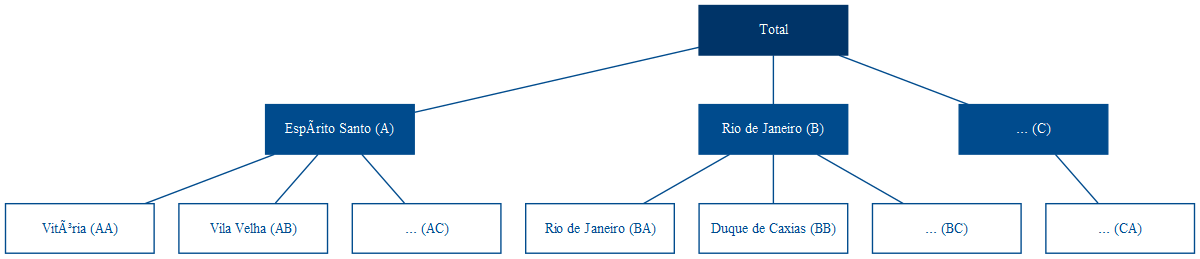
\includegraphics{img/hierarq.png}

}

\caption{\label{fig-h}Séries Hierárquicas}

\end{figure}

Essa estrutura pode ser representada por equações para qualquer nível de
agregação. Assim, o agregado nacional pode ser representado apenas pelos
agregados dos estados, através de \eqref{eq:ha}, ou como o agregado dos
municípios \eqref{eq:ha_mun}. Já o agregado para o estado do Espírito
Santo é representado por \eqref{eq:haES}.

\begin{align}
y_t &= y_{A,t} + y_{B,t} + y_{C,t} \label{eq:ha} \\
y_t &= y_{AA,t} + y_{AB,t} + y_{AC,t} + y_{BA,t} + y_{BC,t} + y_{CA,t}\label{eq:ha_mun} \\
y_{A,t} &= y_{AA,t} + y_{AB,t} + y_{AC,t} \label{eq:haES}
\end{align}

Alternativamente, podemos descrever a estrutura completa de forma
matricial:

\begin{equation}\protect\hypertarget{eq-matriz_hierarquia}{}{
\begin{bmatrix}
    y_{t} \\
    y_{A, t} \\
    y_{B, t} \\
    y_{C, t} \\
    y_{AA, t} \\
    y_{AB, t} \\
    y_{AC, t} \\
    y_{BA, t} \\
    y_{BB, t} \\
    y_{BC, t} \\
    y_{CA, t}
\end{bmatrix}
=
\begin{bmatrix}
    1 & 1 & 1 & 1 & 1 & 1 & 1 \\
    1 & 1 & 1 & 0 & 0 & 0 & 0 \\
    0 & 0 & 0 & 1 & 1 & 1 & 0 \\
    0 & 0 & 0 & 0 & 0 & 0 & 1 \\
    1 & 0 & 0 & 0 & 0 & 0 & 0 \\
    0 & 1 & 0 & 0 & 0 & 0 & 0 \\
    0 & 0 & 1 & 0 & 0 & 0 & 0 \\
    0 & 0 & 0 & 1 & 0 & 0 & 0 \\
    0 & 0 & 0 & 0 & 1 & 0 & 0 \\
    0 & 0 & 0 & 0 & 0 & 1 & 0 \\
    0 & 0 & 0 & 0 & 0 & 0 & 1 \\
\end{bmatrix}
\begin{bmatrix}
    y_{AA, t} \\
    y_{AB, t} \\
    y_{AC, t} \\
    y_{BA, t} \\
    y_{BB, t} \\
    y_{BC, t} \\
    y_{CA, t}
\end{bmatrix}
}\label{eq-matriz_hierarquia}\end{equation}

Por outro lado, o Pib pode ser também desagregado de forma cruzada de
acordo com a atividade econômica --- lavoura, rebanho, indústria de
transformação, extrativa, bens de capital, bens intermediários, comércio
de vestuário, automotivos, serviços etc. Essa estrutura não pode ser
desagregada naturalmente de uma única forma, como é a hierarquia de
estados e municípios. Não pode ser aninhada por um atributo como a
própria geografia. A esse tipo de estrutura dá-se o nome de séries
agrupadas.

\begin{figure}

{\centering 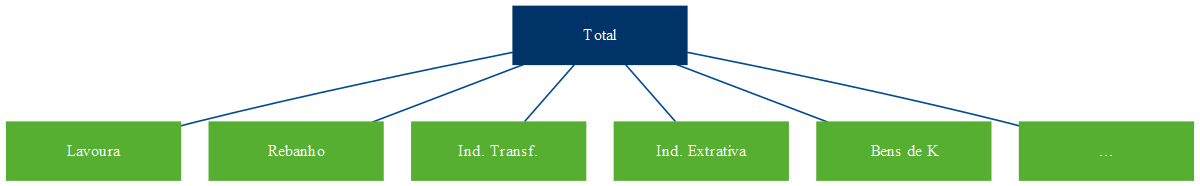
\includegraphics{img/agrupadas.png}

}

\caption{\label{fig-a}Séries Agrupadas}

\end{figure}

Combinando as duas, temos a estrutura de séries hierárquicas agrupadas.
Ao contrário da estrutura hierárquica, que só pode ser agregada de uma
forma --- como com os municípios abaixo dos estados ---, a adição da
estrutura agrupada pode ocorrer tanto acima (figura~\ref{fig-ha1})
quanto abaixo (figura~\ref{fig-ha2}) da hierárquica.

\begin{figure}

{\centering 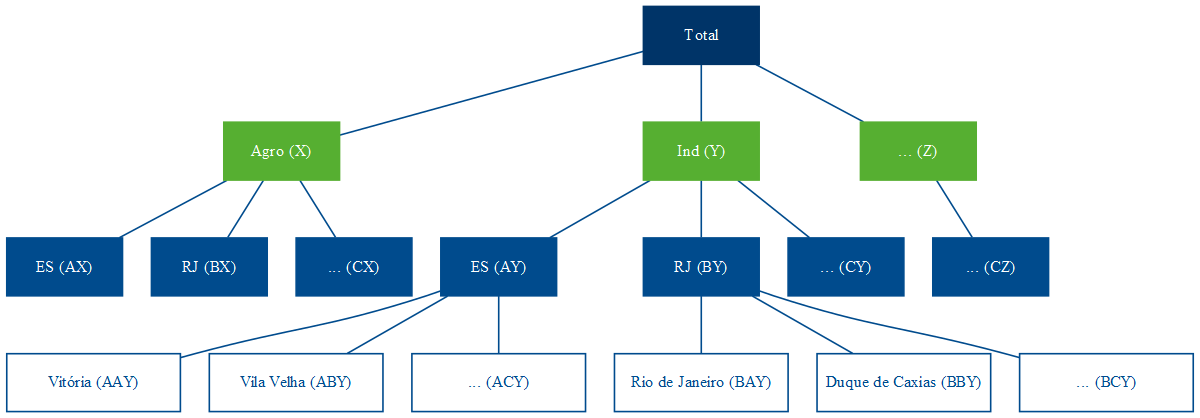
\includegraphics{img/hier_agrup.png}

}

\caption{\label{fig-ha1}Séries Hierárquicas Agrupadas (a)}

\end{figure}

\begin{figure}

{\centering 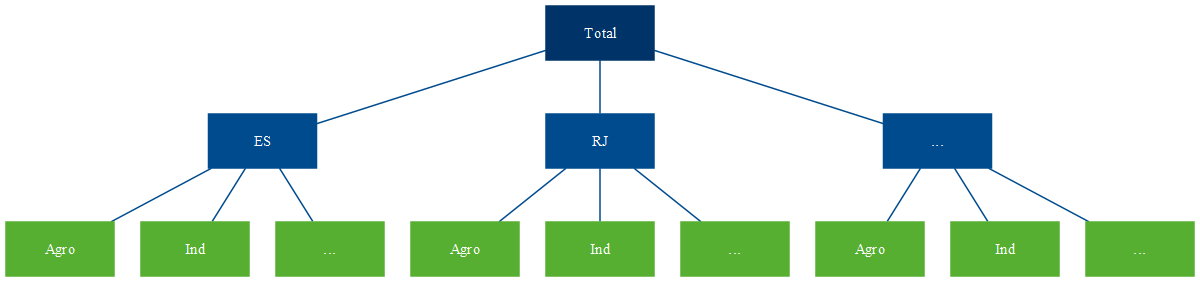
\includegraphics{img/hier_agrup_2.png}

}

\caption{\label{fig-ha2}Séries Hierárquicas Agrupadas (b)}

\end{figure}

Na notação matricial, a estrutura da figura~\ref{fig-ha2} é representada
como abaixo. Formalmente, o primeiro membro da igualdade é composto pelo
vetor \(\mathbfit{y}_t\) \(n\)-dimensional com todas as observações no
tempo \(t\) para todos os níveis da hierarquia. O segundo membro é
composto pela matriz de soma \(\mathbfit{S}\) de dimensão \(n \times m\)
que define as equações para todo nível de agregação, e pela matriz
\(\mathbfit{b}_t\) composta pelas séries no nível mais desagregado.

\[
\mathbfit{y}_t=\mathbfit{Sb}_t
\]

\begin{equation}\protect\hypertarget{eq-matriz_ha}{}{
\begin{bmatrix}
    y_{t} \\
    y_{A, t} \\
    y_{B, t} \\
    y_{C, t} \\
    y_{X, t} \\
    y_{Y, t} \\
    y_{Z, t} \\
    y_{AX, t} \\
    y_{AY, t} \\
    y_{AZ, t} \\
    y_{BX, t} \\
    y_{BY, t} \\
    y_{BZ, t} \\
    y_{CX, t} \\
    y_{CY, t} \\
    y_{CZ, t}
\end{bmatrix}
=
\begin{bmatrix}
    1 & 1 & 1 & 1 & 1 & 1 & 1 & 1 & 1 \\
    1 & 1 & 1 & 0 & 0 & 0 & 0 & 0 & 0 \\
    0 & 0 & 0 & 1 & 1 & 1 & 0 & 0 & 0 \\
    0 & 0 & 0 & 0 & 0 & 0 & 1 & 1 & 1 \\
    1 & 0 & 0 & 1 & 0 & 0 & 1 & 0 & 0 \\
    0 & 1 & 0 & 0 & 1 & 0 & 0 & 1 & 0 \\
    0 & 0 & 1 & 0 & 0 & 1 & 0 & 0 & 1 \\
    1 & 0 & 0 & 0 & 0 & 0 & 0 & 0 & 0 \\
    0 & 1 & 0 & 0 & 0 & 0 & 0 & 0 & 0 \\
    0 & 0 & 1 & 0 & 0 & 0 & 0 & 0 & 0 \\
    0 & 0 & 0 & 1 & 0 & 0 & 0 & 0 & 0 \\
    0 & 0 & 0 & 0 & 1 & 0 & 0 & 0 & 0 \\
    0 & 0 & 0 & 0 & 0 & 1 & 0 & 0 & 0 \\
    0 & 0 & 0 & 0 & 0 & 0 & 1 & 0 & 0 \\
    0 & 0 & 0 & 0 & 0 & 0 & 0 & 1 & 0 \\
    0 & 0 & 0 & 0 & 0 & 0 & 0 & 0 & 1
\end{bmatrix}
\begin{bmatrix}
    y_{AX, t} \\
    y_{AY, t} \\
    y_{AZ, t} \\
    y_{BX, t} \\
    y_{BY, t} \\
    y_{BZ, t} \\
    y_{CX, t} \\
    y_{CY, t} \\
    y_{CZ, t}
\end{bmatrix}
}\label{eq-matriz_ha}\end{equation}

\hypertarget{abordagens-top-down-e-bottom-up}{%
\subsection*{ABORDAGENS TOP-DOWN E
BOTTOM-UP}\label{abordagens-top-down-e-bottom-up}}
\addcontentsline{toc}{subsection}{ABORDAGENS TOP-DOWN E BOTTOM-UP}

Talvez as formas mais intuitivas de se pensar em previsões para esses
tipos de estrutura sejam as abordagens top-down e bottom-up. Tome a
estrutura descrita na figura~\ref{fig-h}, por exemplo. Podemos realizar
a previsão para o horizonte de tempo \(h\) do agregado do Pib
brasileiro, representado no topo da hierarquia por \emph{Total}
(\ref{eq-topdown_1}), e então distribuir os valores previstos
proporcionalmente entre os estados e municípios.

\begin{equation}\protect\hypertarget{eq-topdown_1}{}{
\hat{y}_{T+h | T} = E[y_{T+h} | \Omega_T]
}\label{eq-topdown_1}\end{equation}

Essa é a abordagem top-down. Nela, a previsão para os níveis mais
desagregados da hierarquia são determinadas por uma proporção \(p_i\) do
nível agregado. Por exemplo, as previsões para Vitória são dadas pela
equação \ref{eq-topdown_2}.

\begin{equation}\protect\hypertarget{eq-topdown_2}{}{
\tilde{y}_{AA, T+h | T} = p_{1}\hat{y}_{T+h | T}
}\label{eq-topdown_2}\end{equation}

Para isso, temos de definir uma matriz com todos esses pesos, que,
seguindo a formulação de \citet{hyndman2021}, vamos chamar de
\(\mathbfit{G}\):

\begin{equation}\protect\hypertarget{eq-matriz_g}{}{
\mathbfit{G}
=
\begin{bmatrix}
    p_1 & 0 & 0 & 0 & 0 & 0 & 0 & 0 \\
    p_2 & 0 & 0 & 0 & 0 & 0 & 0 & 0 \\
    p_3 & 0 & 0 & 0 & 0 & 0 & 0 & 0 \\
    p_4 & 0 & 0 & 0 & 0 & 0 & 0 & 0 \\
    p_5 & 0 & 0 & 0 & 0 & 0 & 0 & 0
\end{bmatrix}
}\label{eq-matriz_g}\end{equation}

\(\mathbfit{G}\) é uma matriz \(m \times n\) que multiplica a matriz
\(\hat{\mathbfit{y}}_{T+h|T}\) que, por sua vez, é composta pelas
previsões base --- as previsões para todos os níveis de agregação. A
equação para a abordagem \emph{top-down} será, então:

\begin{equation}\protect\hypertarget{eq-topdown_3}{}{
\mathbfit{\tilde{y}}_{T+h | T} = \mathbfit{SG\hat{y}}_{T+h | T}
}\label{eq-topdown_3}\end{equation}

Na notação matricial para a estrutura da figura~\ref{fig-h}, temos:

\begin{equation}\protect\hypertarget{eq-matriz_topdown1}{}{
\begin{bmatrix}
    \tilde{y}_{t} \\
    \tilde{y}_{A, t} \\
    \tilde{y}_{B, t} \\
    \tilde{y}_{C, t} \\
    \tilde{y}_{AA, t} \\
    \tilde{y}_{AB, t} \\
    \tilde{y}_{AC, t} \\
    \tilde{y}_{BA, t} \\
    \tilde{y}_{BB, t} \\
    \tilde{y}_{BC, t} \\
    \tilde{y}_{CA, t}
\end{bmatrix}
=
\mathbfit{S}
\begin{bmatrix}
    p_1 & 0 & 0 & 0 & 0 & 0 & 0 & 0 & 0 & 0 & 0 \\
    p_2 & 0 & 0 & 0 & 0 & 0 & 0 & 0 & 0 & 0 & 0 \\
    p_3 & 0 & 0 & 0 & 0 & 0 & 0 & 0 & 0 & 0 & 0 \\
    p_4 & 0 & 0 & 0 & 0 & 0 & 0 & 0 & 0 & 0 & 0 \\
    p_5 & 0 & 0 & 0 & 0 & 0 & 0 & 0 & 0 & 0 & 0 \\
    p_6 & 0 & 0 & 0 & 0 & 0 & 0 & 0 & 0 & 0 & 0 \\
    p_7 & 0 & 0 & 0 & 0 & 0 & 0 & 0 & 0 & 0 & 0 \\
    p_8 & 0 & 0 & 0 & 0 & 0 & 0 & 0 & 0 & 0 & 0 \\
    p_9 & 0 & 0 & 0 & 0 & 0 & 0 & 0 & 0 & 0 & 0 \\
    p_{10} & 0 & 0 & 0 & 0 & 0 & 0 & 0 & 0 & 0 & 0 \\
    p_{11} & 0 & 0 & 0 & 0 & 0 & 0 & 0 & 0 & 0 & 0
\end{bmatrix}
\begin{bmatrix}
    \hat{y}_{T+h|T} \\
    \hat{y}_{A, T+h|T} \\
    \hat{y}_{B, T+h|T} \\
    \hat{y}_{C, T+h|T} \\
    \hat{y}_{AA, T+h|T} \\
    \hat{y}_{AB, T+h|T} \\
    \hat{y}_{AC, T+h|T} \\
    \hat{y}_{BA, T+h|T} \\
    \hat{y}_{BB, T+h|T} \\
    \hat{y}_{BC, T+h|T} \\
    \hat{y}_{CA, T+h|T}
\end{bmatrix}
}\label{eq-matriz_topdown1}\end{equation}

\begin{equation}\protect\hypertarget{eq-matriz_topdown2}{}{
\begin{bmatrix}
    \tilde{y}_{t} \\
    \tilde{y}_{A, t} \\
    \tilde{y}_{B, t} \\
    \tilde{y}_{C, t} \\
    \tilde{y}_{AA, t} \\
    \tilde{y}_{AB, t} \\
    \tilde{y}_{AC, t} \\
    \tilde{y}_{BA, t} \\
    \tilde{y}_{BB, t} \\
    \tilde{y}_{BC, t} \\
    \tilde{y}_{CA, t}
\end{bmatrix}
=
\mathbfit{S}
\begin{bmatrix}
    p_1\hat{y}_{T+h|T} \\
    p_2\hat{y}_{T+h|T} \\
    p_3\hat{y}_{T+h|T} \\
    p_4\hat{y}_{T+h|T} \\
    p_5\hat{y}_{T+h|T} \\
    p_6\hat{y}_{T+h|T} \\
    p_7\hat{y}_{T+h|T} \\
    p_8\hat{y}_{T+h|T} \\
    p_9\hat{y}_{T+h|T} \\
    p_{10}\hat{y}_{T+h|T} \\
    p_{11}\hat{y}_{T+h|T}
\end{bmatrix}
}\label{eq-matriz_topdown2}\end{equation}

A matriz \(\mathbfit{S}\) aqui será, temos:

\begin{equation}\protect\hypertarget{eq-matriz_topdown3}{}{
\begin{bmatrix}
    \tilde{y}_{t} \\
    \tilde{y}_{A, t} \\
    \tilde{y}_{B, t} \\
    \tilde{y}_{C, t} \\
    \tilde{y}_{AA, t} \\
    \tilde{y}_{AB, t} \\
    \tilde{y}_{AC, t} \\
    \tilde{y}_{BA, t} \\
    \tilde{y}_{BB, t} \\
    \tilde{y}_{BC, t} \\
    \tilde{y}_{CA, t}
\end{bmatrix}
=
\begin{bmatrix}
    0 & 0 & 0 & 0 & 0 & 0 & 0 & 1 & 1 & 1 & 1 \\
    0 & 0 & 0 & 0 & 1 & 1 & 1 & 0 & 0 & 0 & 0 \\
    0 & 0 & 0 & 0 & 0 & 0 & 0 & 1 & 1 & 1 & 0 \\
    0 & 0 & 0 & 0 & 0 & 0 & 0 & 0 & 0 & 0 & 1 \\
    0 & 0 & 0 & 0 & 1 & 0 & 0 & 0 & 0 & 0 & 0 \\
    0 & 0 & 0 & 0 & 0 & 1 & 0 & 0 & 0 & 0 & 0 \\
    0 & 0 & 0 & 0 & 0 & 0 & 1 & 0 & 0 & 0 & 0 \\
    0 & 0 & 0 & 0 & 0 & 0 & 0 & 1 & 0 & 0 & 0 \\
    0 & 0 & 0 & 0 & 0 & 0 & 0 & 0 & 1 & 0 & 0 \\
    0 & 0 & 0 & 0 & 0 & 0 & 0 & 0 & 0 & 1 & 0 \\
    0 & 0 & 0 & 0 & 0 & 0 & 0 & 0 & 0 & 0 & 1 \\
\end{bmatrix}
\begin{bmatrix}
    p_1\hat{y}_{T+h|T} \\
    p_2\hat{y}_{T+h|T} \\
    p_3\hat{y}_{T+h|T} \\
    p_4\hat{y}_{T+h|T} \\
    p_5\hat{y}_{T+h|T} \\
    p_6\hat{y}_{T+h|T} \\
    p_7\hat{y}_{T+h|T} \\
    p_8\hat{y}_{T+h|T} \\
    p_9\hat{y}_{T+h|T} \\
    p_{10}\hat{y}_{T+h|T} \\
    p_{11}\hat{y}_{T+h|T}
\end{bmatrix}
}\label{eq-matriz_topdown3}\end{equation}

\newpage

\hypertarget{revisuxe3o-da-literatura}{%
\section{REVISÃO DA LITERATURA}\label{revisuxe3o-da-literatura}}

\newpage

\hypertarget{referuxeancias}{%
\section*{REFERÊNCIAS}\label{referuxeancias}}
\addcontentsline{toc}{section}{REFERÊNCIAS}

\bibliography{config/bib.bib, config/packages.bib}



\end{document}
